% MULTI-PAGE GRAPHICS IN LATEX - COMPLETE GUIDE

% ==================================================================
% METHOD 1: Native LaTeX Multi-Page Solution (RECOMMENDED)
% ==================================================================
% This is the best approach for academic thesis work

% To include the multi-page user flow in your thesis, simply uncomment this line in methodology.tex:
% % Multi-page TikZ User Flow for LaTeX
% This creates a user flow that spans multiple pages naturally

\clearpage
\subsection{Detailed User Flow Documentation}

The complete Consol user flow requires detailed documentation across multiple operational phases. The following pages present comprehensive flow diagrams for each major system component.

\subsubsection{Phase 1: Authentication and Initial Setup}

\begin{figure}[H]
\centering
\begin{tikzpicture}[
    node distance=1.5cm,
    every node/.style={align=center},
    start/.style={ellipse, draw=green!60, fill=green!20, thick, minimum width=2.5cm, minimum height=1cm},
    process/.style={rectangle, draw=blue!60, fill=blue!20, thick, minimum width=2.8cm, minimum height=1.2cm, rounded corners=3pt},
    decision/.style={diamond, draw=red!60, fill=red!20, thick, minimum width=2cm, minimum height=1cm},
    data/.style={trapezium, draw=purple!60, fill=purple!20, thick, minimum width=2.5cm, minimum height=1cm},
    system/.style={rectangle, draw=orange!60, fill=orange!20, thick, minimum width=2.8cm, minimum height=1.2cm}
]

% Authentication flow
\node[start] (start) at (0,0) {User Accesses\\Consol System};
\node[system] (auth) at (0,-2) {System\\Authentication\\Check};
\node[decision] (logged) at (0,-4) {User\\Logged In?};

% Login branch
\node[process] (login) at (-4,-6) {Display Login\\Interface};
\node[decision] (account) at (-4,-8) {Has Account?};
\node[process] (register) at (-6,-10) {Registration\\Form};
\node[process] (submit) at (-2,-10) {Login\\Submission};

% Dashboard setup
\node[process] (dashboard) at (0,-12) {Load Main\\Dashboard};
\node[data] (userdata) at (3,-12) {Fetch User\\Profile};
\node[system] (interface) at (0,-14) {Initialize\\Interface};

% Phase completion
\node[system] (complete) at (0,-16) {Continue to\\Action Selection};

% Connections
\draw[thick,->] (start) -- (auth);
\draw[thick,->] (auth) -- (logged);
\draw[thick,->] (logged) -- node[left] {No} (login);
\draw[thick,->] (logged) -- node[right] {Yes} (dashboard);
\draw[thick,->] (login) -- (account);
\draw[thick,->] (account) -- node[left] {No} (register);
\draw[thick,->] (account) -- node[right] {Yes} (submit);
\draw[thick,->] (register) -- (dashboard);
\draw[thick,->] (submit) -- (dashboard);
\draw[thick,->] (dashboard) -- (userdata);
\draw[thick,->] (dashboard) -- (interface);
\draw[thick,->] (interface) -- (complete);

\end{tikzpicture}
\caption{User Authentication and Dashboard Setup Flow}
\label{fig:userflow-auth}
\end{figure}

This phase establishes user identity and prepares the personalized learning environment. The system verifies credentials, handles new user registration, and initializes the dashboard with user-specific data and interface elements.

\clearpage
\subsubsection{Phase 2: Note Management Operations}

\begin{figure}[H]
\centering
\begin{tikzpicture}[
    node distance=1.5cm,
    every node/.style={align=center},
    start/.style={ellipse, draw=green!60, fill=green!20, thick, minimum width=2.5cm, minimum height=1cm},
    process/.style={rectangle, draw=blue!60, fill=blue!20, thick, minimum width=2.8cm, minimum height=1.2cm, rounded corners=3pt},
    decision/.style={diamond, draw=red!60, fill=red!20, thick, minimum width=2cm, minimum height=1cm},
    data/.style={trapezium, draw=purple!60, fill=purple!20, thick, minimum width=2.5cm, minimum height=1cm}
]

% Entry point
\node[start] (entry) at (0,0) {From Dashboard\\Action Selection};
\node[decision] (action) at (0,-2) {User\\Action?};

% Note creation branch (left)
\node[process] (create) at (-4,-4) {Create New\\Note};
\node[process] (input) at (-4,-6) {Text Input\\Interface};
\node[data] (validate) at (-4,-8) {Content\\Validation};
\node[decision] (valid) at (-4,-10) {Text Valid?};
\node[process] (error) at (-6,-12) {Show Error\\Message};
\node[data] (embed) at (-4,-14) {SimCSE\\Processing};
\node[data] (store) at (-4,-16) {Database\\Storage};

% Note management branch (right)
\node[process] (manage) at (4,-4) {Manage\\Notes};
\node[process] (list) at (4,-6) {Display\\Notes List};
\node[decision] (noteaction) at (4,-8) {Note\\Action?};
\node[process] (edit) at (2,-10) {Edit\\Note};
\node[process] (delete) at (6,-10) {Delete\\Note};
\node[data] (update) at (4,-12) {Update\\Database};

% Completion
\node[start] (next) at (0,-18) {Continue to Practice\\or Analytics};

% Connections - Creation branch
\draw[thick,->] (entry) -- (action);
\draw[thick,->] (action) -- node[left] {Create} (create);
\draw[thick,->] (create) -- (input);
\draw[thick,->] (input) -- (validate);
\draw[thick,->] (validate) -- (valid);
\draw[thick,->] (valid) -- node[left] {No} (error);
\draw[thick,->] (valid) -- node[right] {Yes} (embed);
\draw[thick,->] (error) -- (input);
\draw[thick,->] (embed) -- (store);
\draw[thick,->] (store) -- (next);

% Connections - Management branch
\draw[thick,->] (action) -- node[right] {Manage} (manage);
\draw[thick,->] (manage) -- (list);
\draw[thick,->] (list) -- (noteaction);
\draw[thick,->] (noteaction) -- node[left] {Edit} (edit);
\draw[thick,->] (noteaction) -- node[right] {Delete} (delete);
\draw[thick,->] (edit) -- (update);
\draw[thick,->] (delete) -- (update);
\draw[thick,->] (update) -- (next);

\end{tikzpicture}
\caption{Note Creation and Management Workflow}
\label{fig:userflow-notes}
\end{figure}

This phase handles all content management operations. Users can create new learning notes with automatic validation and SimCSE preprocessing, or manage existing notes through editing and deletion operations with appropriate database updates.

\clearpage
\subsubsection{Phase 3: Practice Session Execution}

\begin{figure}[H]
\centering
\begin{tikzpicture}[
    node distance=1.5cm,
    every node/.style={align=center},
    start/.style={ellipse, draw=green!60, fill=green!20, thick, minimum width=2.5cm, minimum height=1cm},
    process/.style={rectangle, draw=blue!60, fill=blue!20, thick, minimum width=2.8cm, minimum height=1.2cm, rounded corners=3pt},
    decision/.style={diamond, draw=red!60, fill=red!20, thick, minimum width=2cm, minimum height=1cm},
    data/.style={trapezium, draw=purple!60, fill=purple!20, thick, minimum width=2.5cm, minimum height=1cm},
    system/.style={rectangle, draw=orange!60, fill=orange!20, thick, minimum width=2.8cm, minimum height=1.2cm}
]

% Practice session start
\node[start] (start) at (0,0) {Begin Practice\\Session};
\node[process] (select) at (0,-2) {Select Note\\for Practice};
\node[process] (display) at (0,-4) {Display Original\\Text Prompt};
\node[system] (timer) at (0,-6) {Start Session\\Timer};
\node[process] (input) at (0,-8) {User Types\\Recall Response};

% Session decision point
\node[decision] (complete) at (0,-10) {Session\\Complete?};

% Hint system (left branch)
\node[process] (hint) at (-4,-12) {Provide Hint\\to User};
\node[data] (counter) at (-4,-14) {Increment\\Hint Counter};

% Assessment processing (right branch)
\node[system] (stop) at (4,-12) {Stop Timer\\Calculate Duration};
\node[data] (similarity) at (4,-14) {SimCSE Similarity\\Calculation};
\node[data] (metrics) at (4,-16) {Performance\\Evaluation};
\node[data] (rating) at (4,-18) {Star Rating\\Generation};

% Results display
\node[process] (results) at (0,-20) {Display Results\\and Feedback};
\node[start] (end) at (0,-22) {Session Assessment\\Complete};

% Connections
\draw[thick,->] (start) -- (select);
\draw[thick,->] (select) -- (display);
\draw[thick,->] (display) -- (timer);
\draw[thick,->] (timer) -- (input);
\draw[thick,->] (input) -- (complete);

% Hint branch
\draw[thick,->] (complete) -- node[left] {Need Hint} (hint);
\draw[thick,->] (hint) -- (counter);
\draw[thick,->] (counter) -- (input);

% Assessment branch
\draw[thick,->] (complete) -- node[right] {Complete} (stop);
\draw[thick,->] (stop) -- (similarity);
\draw[thick,->] (similarity) -- (metrics);
\draw[thick,->] (metrics) -- (rating);
\draw[thick,->] (rating) -- (results);
\draw[thick,->] (results) -- (end);

\end{tikzpicture}
\caption{Practice Session Workflow and Assessment}
\label{fig:userflow-practice}
\end{figure}

This phase manages the core assessment functionality. Users engage with selected notes through timed recall exercises, receive hints when needed, and undergo comprehensive performance evaluation using SimCSE similarity analysis with multi-dimensional feedback generation.

\clearpage
\subsubsection{Phase 4: Analytics and Session Management}

\begin{figure}[H]
\centering
\begin{tikzpicture}[
    node distance=1.5cm,
    every node/.style={align=center},
    start/.style={ellipse, draw=green!60, fill=green!20, thick, minimum width=2.5cm, minimum height=1cm},
    process/.style={rectangle, draw=blue!60, fill=blue!20, thick, minimum width=2.8cm, minimum height=1.2cm, rounded corners=3pt},
    decision/.style={diamond, draw=red!60, fill=red!20, thick, minimum width=2cm, minimum height=1cm},
    data/.style={trapezium, draw=purple!60, fill=purple!20, thick, minimum width=2.5cm, minimum height=1cm}
]

% Session continuation decision
\node[start] (continue_start) at (0,0) {After Practice\\Session};
\node[decision] (continue) at (0,-2) {Continue\\Practice?};

% Practice continuation (left)
\node[process] (newpractice) at (-4,-4) {Select Different\\Note};
\node[process] (backpractice) at (-4,-6) {Return to Practice\\Flow};

% Analytics branch (right)
\node[process] (analytics) at (4,-4) {View Progress\\Analytics};
\node[process] (dashboard) at (4,-6) {Load Analytics\\Dashboard};
\node[data] (trends) at (2,-8) {Calculate\\Learning Trends};
\node[data] (charts) at (6,-8) {Generate\\Progress Charts};
\node[process] (analysis) at (4,-10) {Display Detailed\\Analysis};

% Export functionality
\node[decision] (export) at (4,-12) {Export\\Data?};
\node[process] (report) at (2,-14) {Generate PDF\\Report};

% Session completion
\node[data] (store) at (0,-16) {Store Session\\in Database};
\node[data] (progress) at (0,-18) {Update User\\Progress};
\node[process] (dashboard_return) at (0,-20) {Return to Main\\Dashboard};
\node[start] (end) at (0,-22) {Session\\Complete};

% Connections
\draw[thick,->] (continue_start) -- (continue);
\draw[thick,->] (continue) -- node[left] {Yes} (newpractice);
\draw[thick,->] (continue) -- node[right] {No} (analytics);
\draw[thick,->] (newpractice) -- (backpractice);
\draw[thick,->] (backpractice) -- (continue);

% Analytics flow
\draw[thick,->] (analytics) -- (dashboard);
\draw[thick,->] (dashboard) -- (trends);
\draw[thick,->] (dashboard) -- (charts);
\draw[thick,->] (trends) -- (analysis);
\draw[thick,->] (charts) -- (analysis);
\draw[thick,->] (analysis) -- (export);
\draw[thick,->] (export) -- node[left] {Yes} (report);
\draw[thick,->] (export) -- node[right] {No} (store);
\draw[thick,->] (report) -- (store);

% Completion flow
\draw[thick,->] (store) -- (progress);
\draw[thick,->] (progress) -- (dashboard_return);
\draw[thick,->] (dashboard_return) -- (end);

\end{tikzpicture}
\caption{Analytics Dashboard and Session Completion}
\label{fig:userflow-analytics}
\end{figure}

This final phase handles session continuation decisions, comprehensive learning analytics, and system state management. Users can continue practicing, analyze their performance through detailed dashboards, export progress reports, and complete their learning sessions with full data persistence.

% This will automatically span across multiple pages with proper page breaks and figure numbering.

% ==================================================================
% METHOD 2: PNG Images Across Multiple Figures
% ==================================================================

% If you prefer to use the PNG images, include them like this:

\begin{figure}[H]
\centering
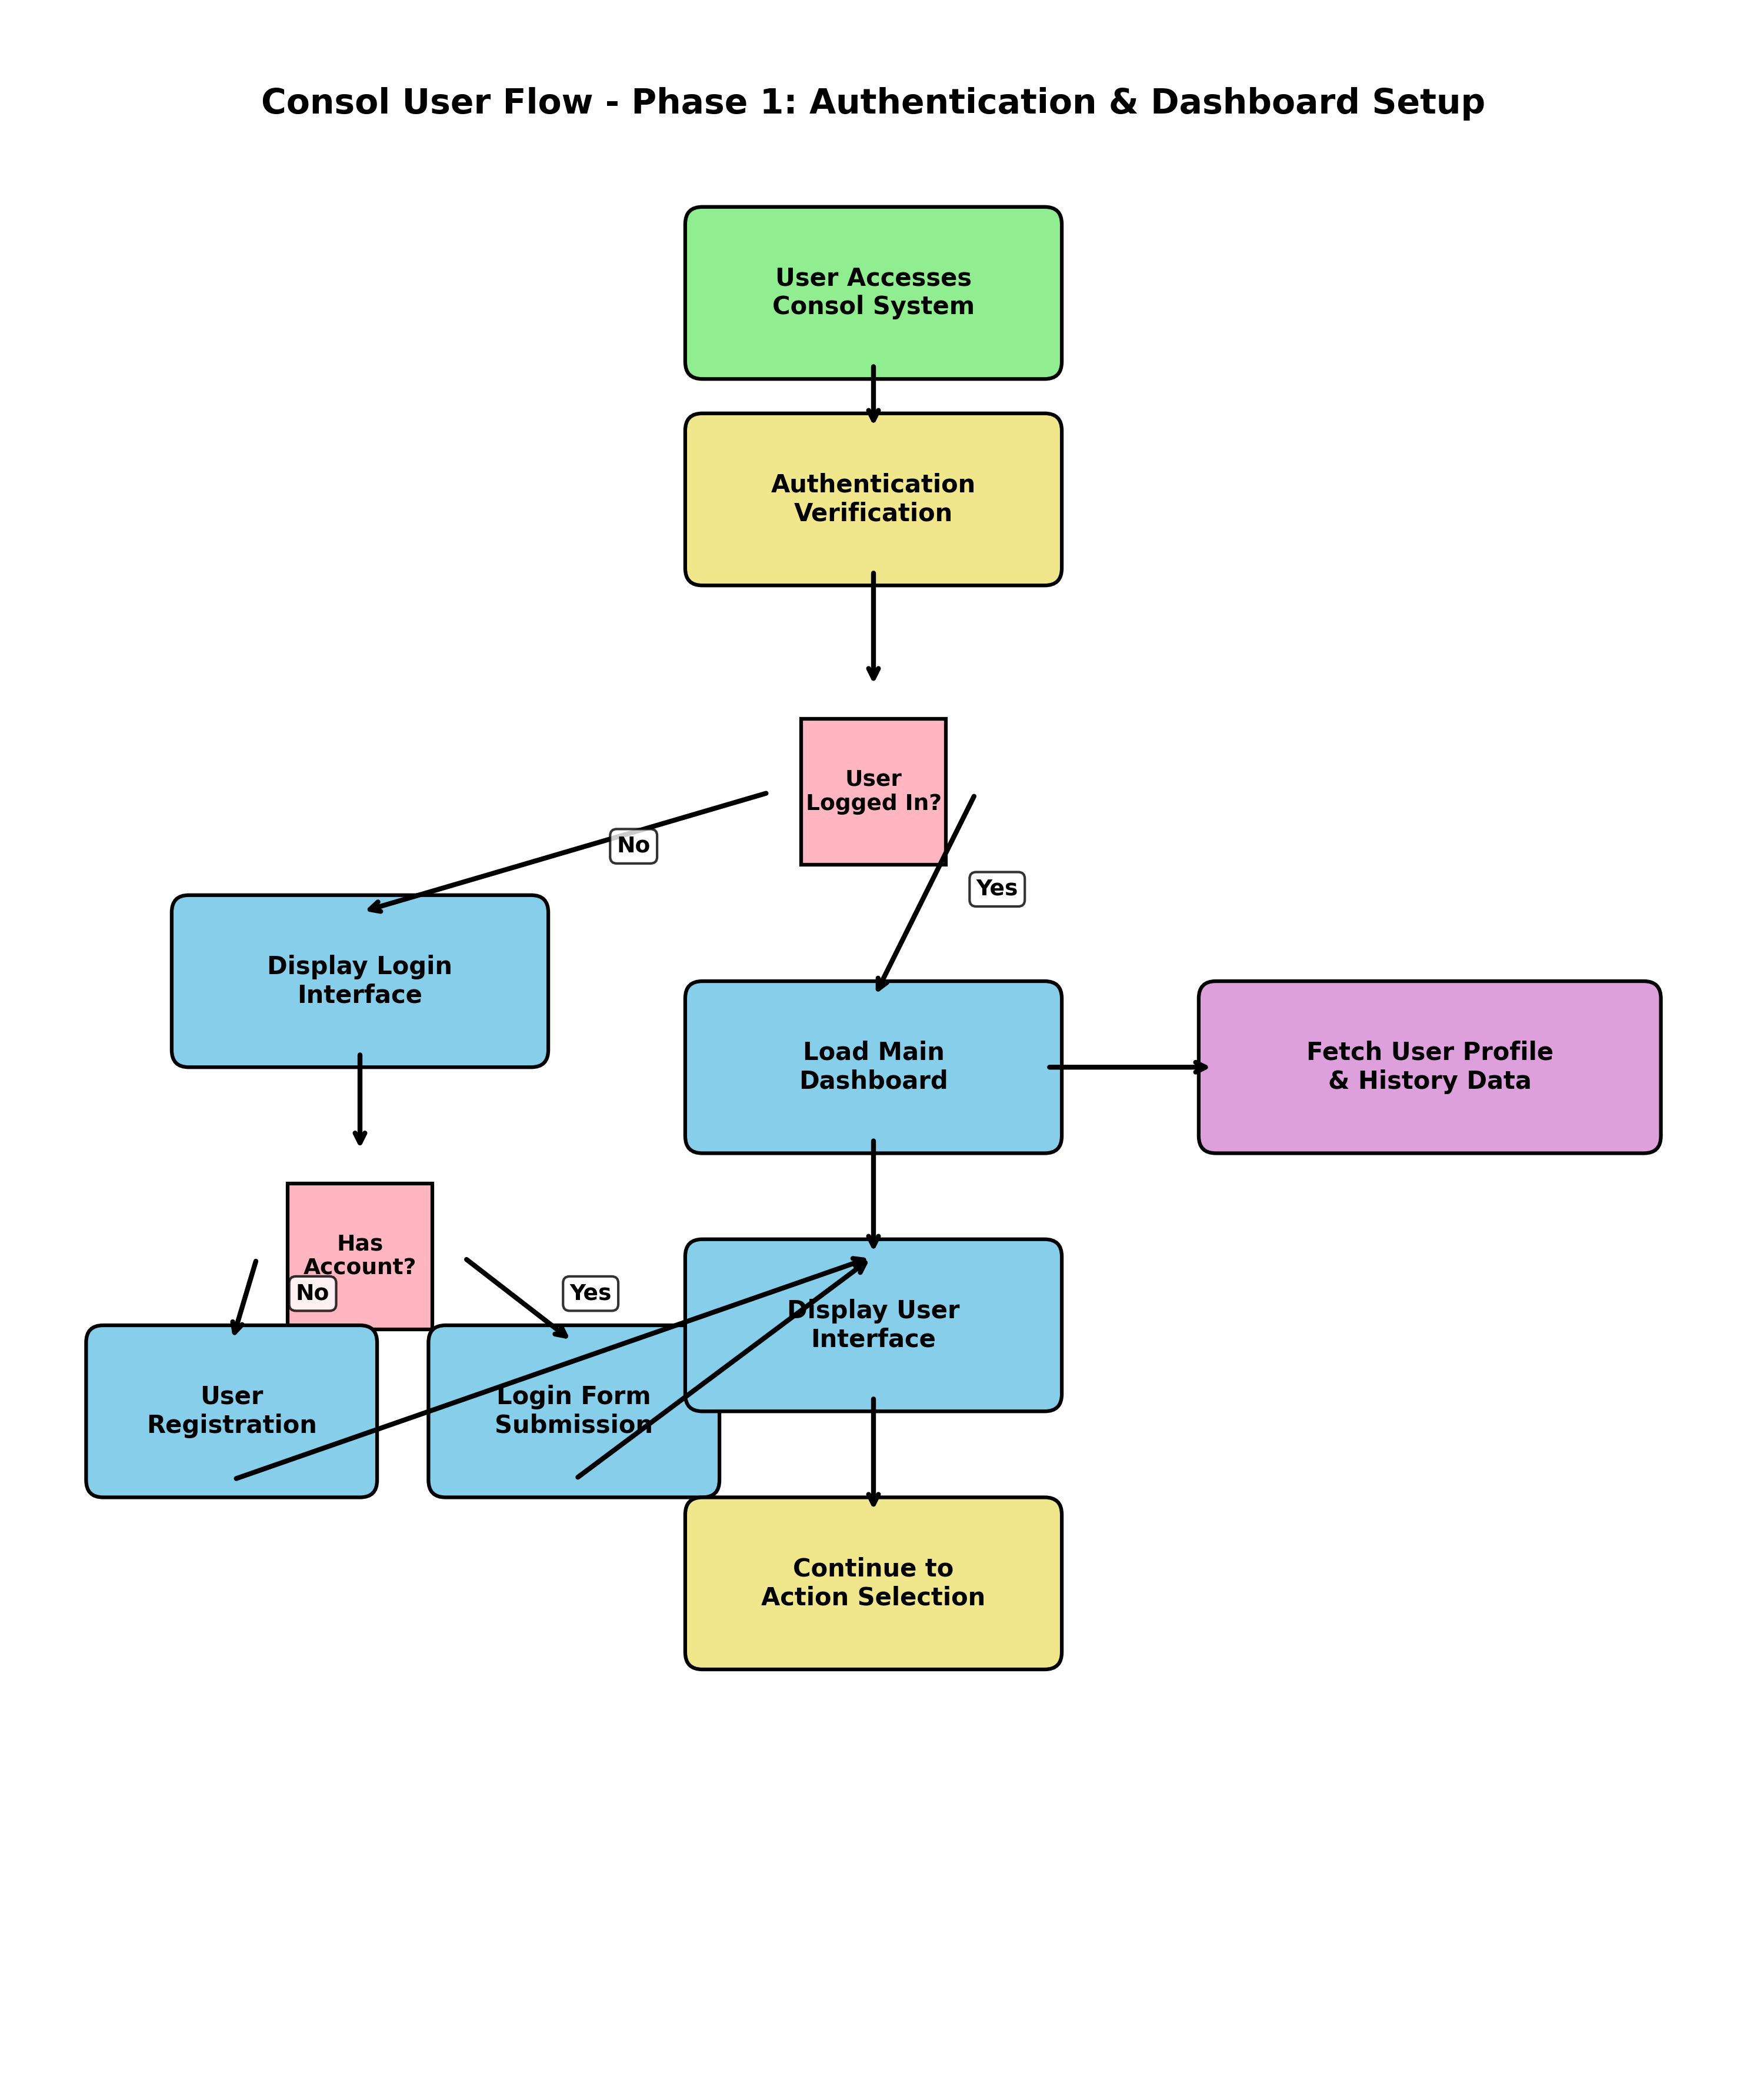
\includegraphics[width=\textwidth]{images/userflow_page1.png}
\caption{User Flow Phase 1: Authentication and Dashboard Setup}
\label{fig:userflow-phase1}
\end{figure}

\begin{figure}[H]
\centering
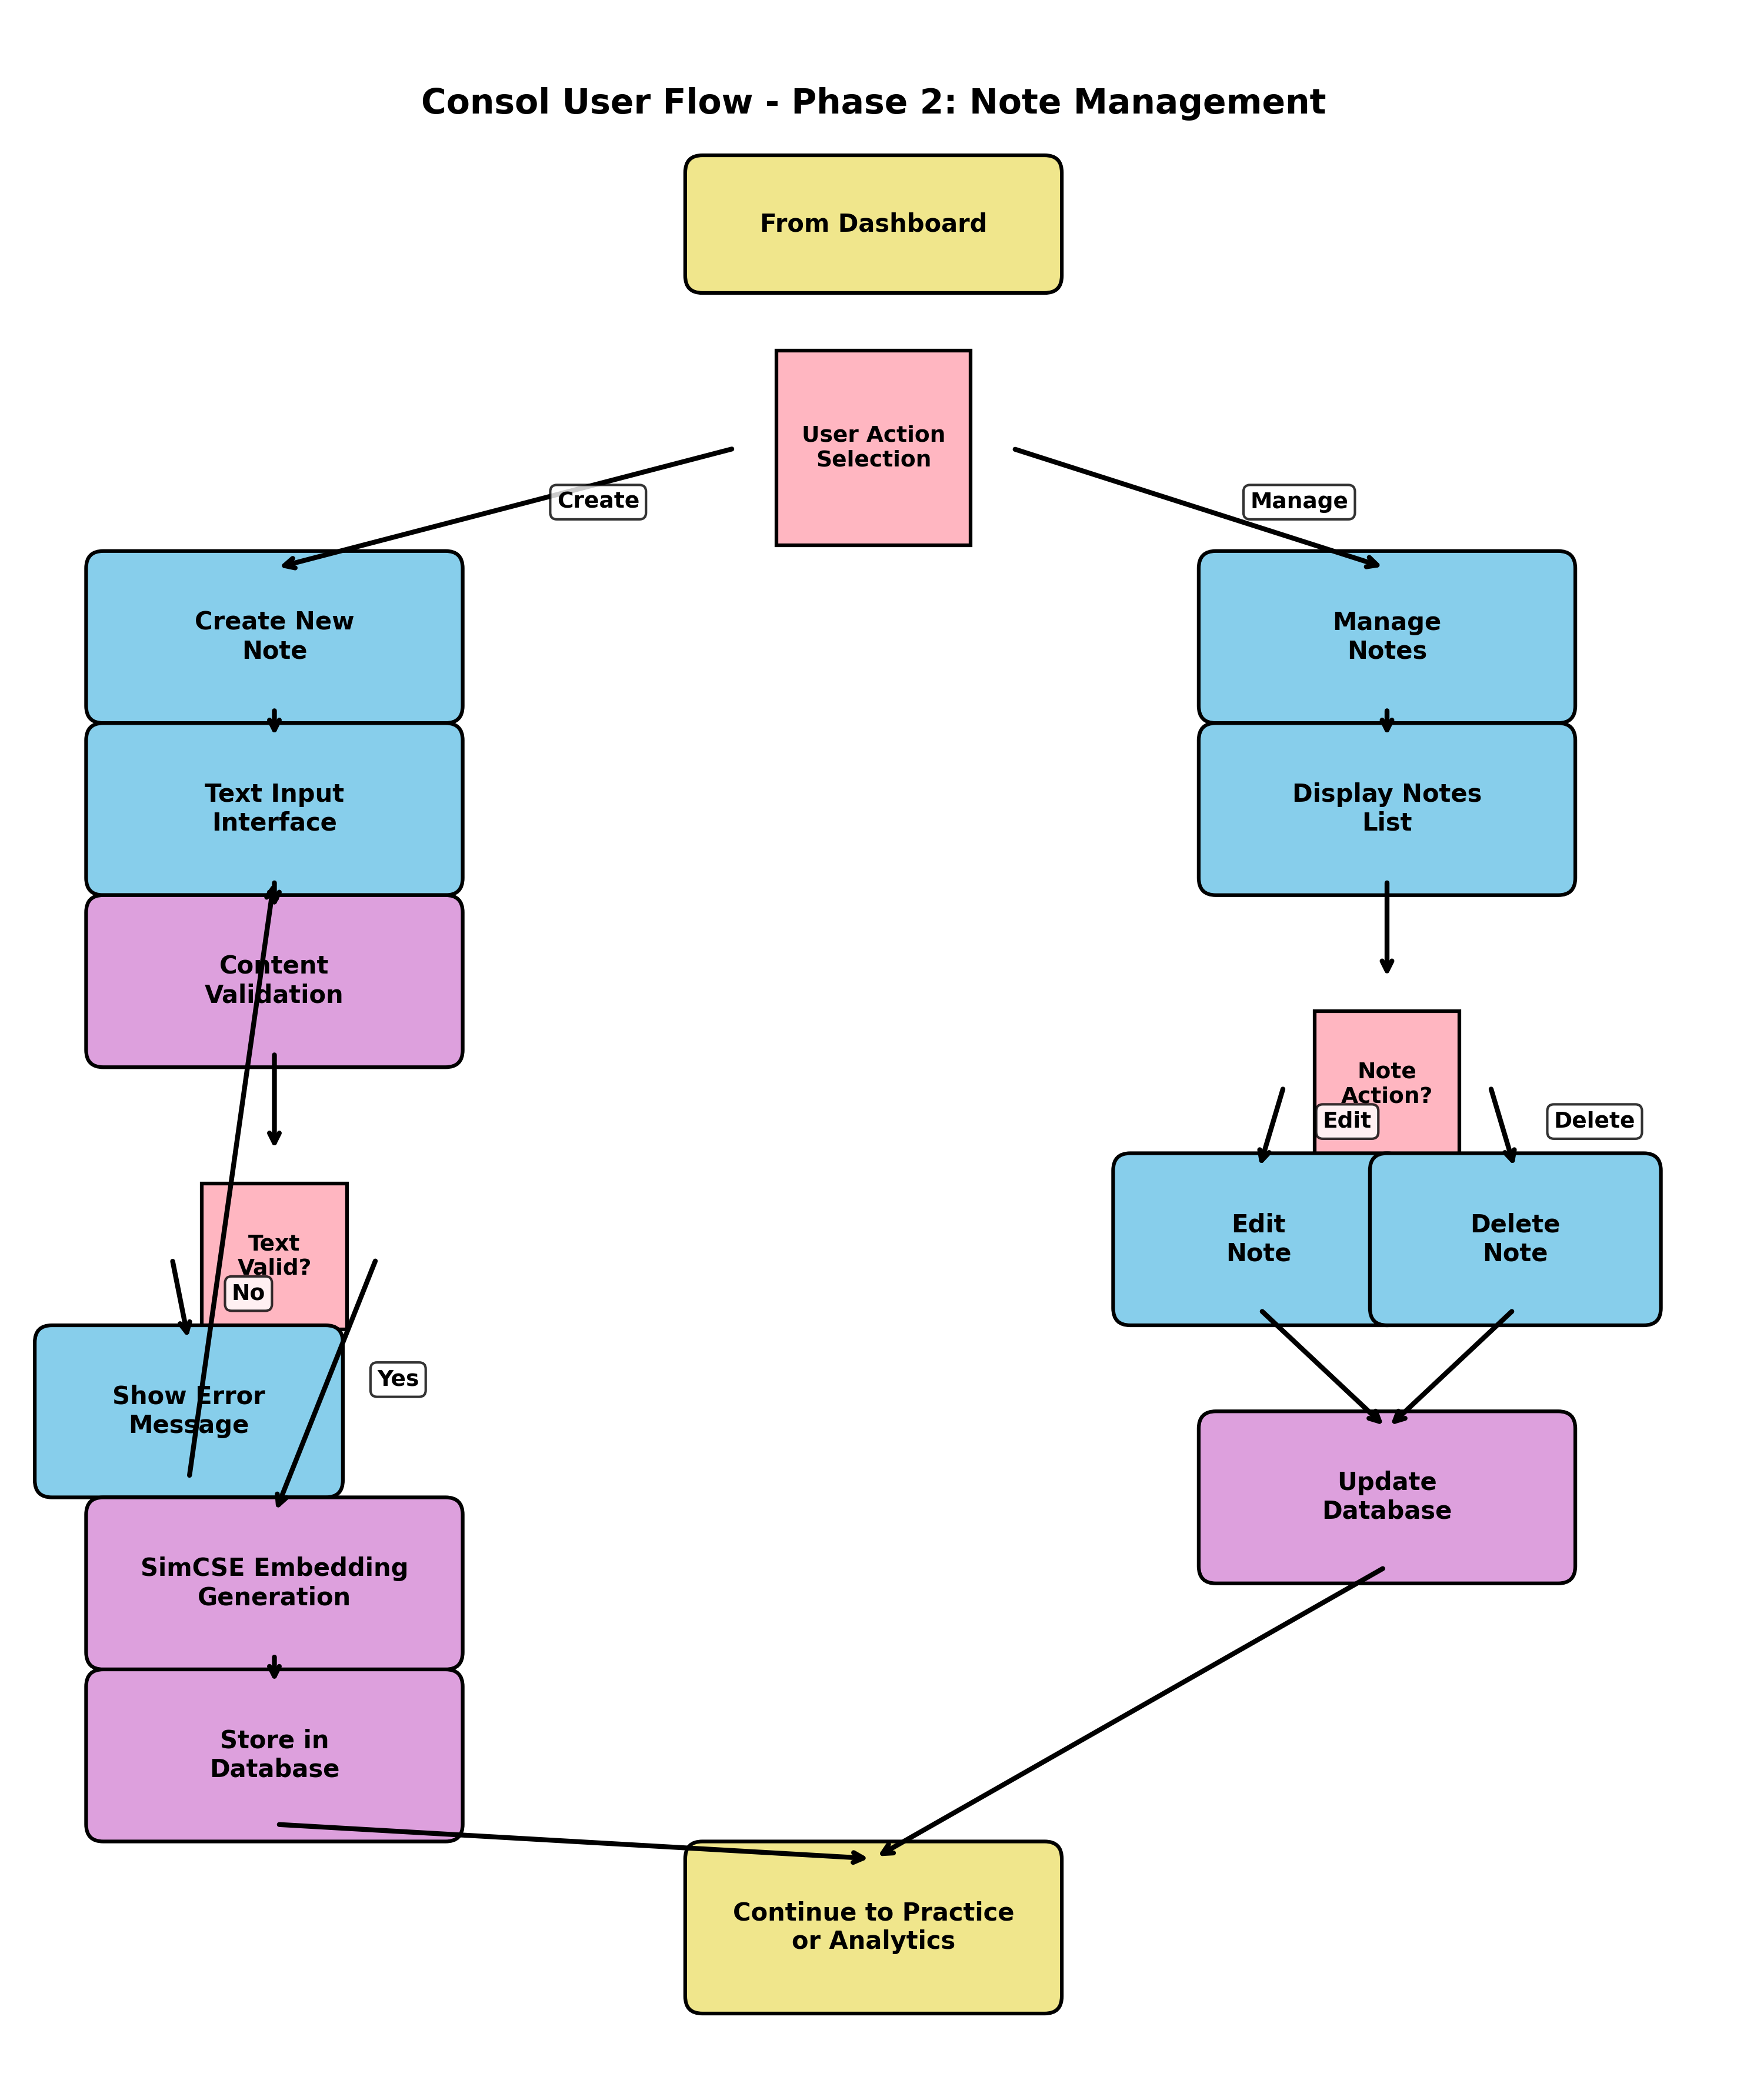
\includegraphics[width=\textwidth]{images/userflow_page2.png}
\caption{User Flow Phase 2: Note Management Operations}
\label{fig:userflow-phase2}
\end{figure}

\begin{figure}[H]
\centering
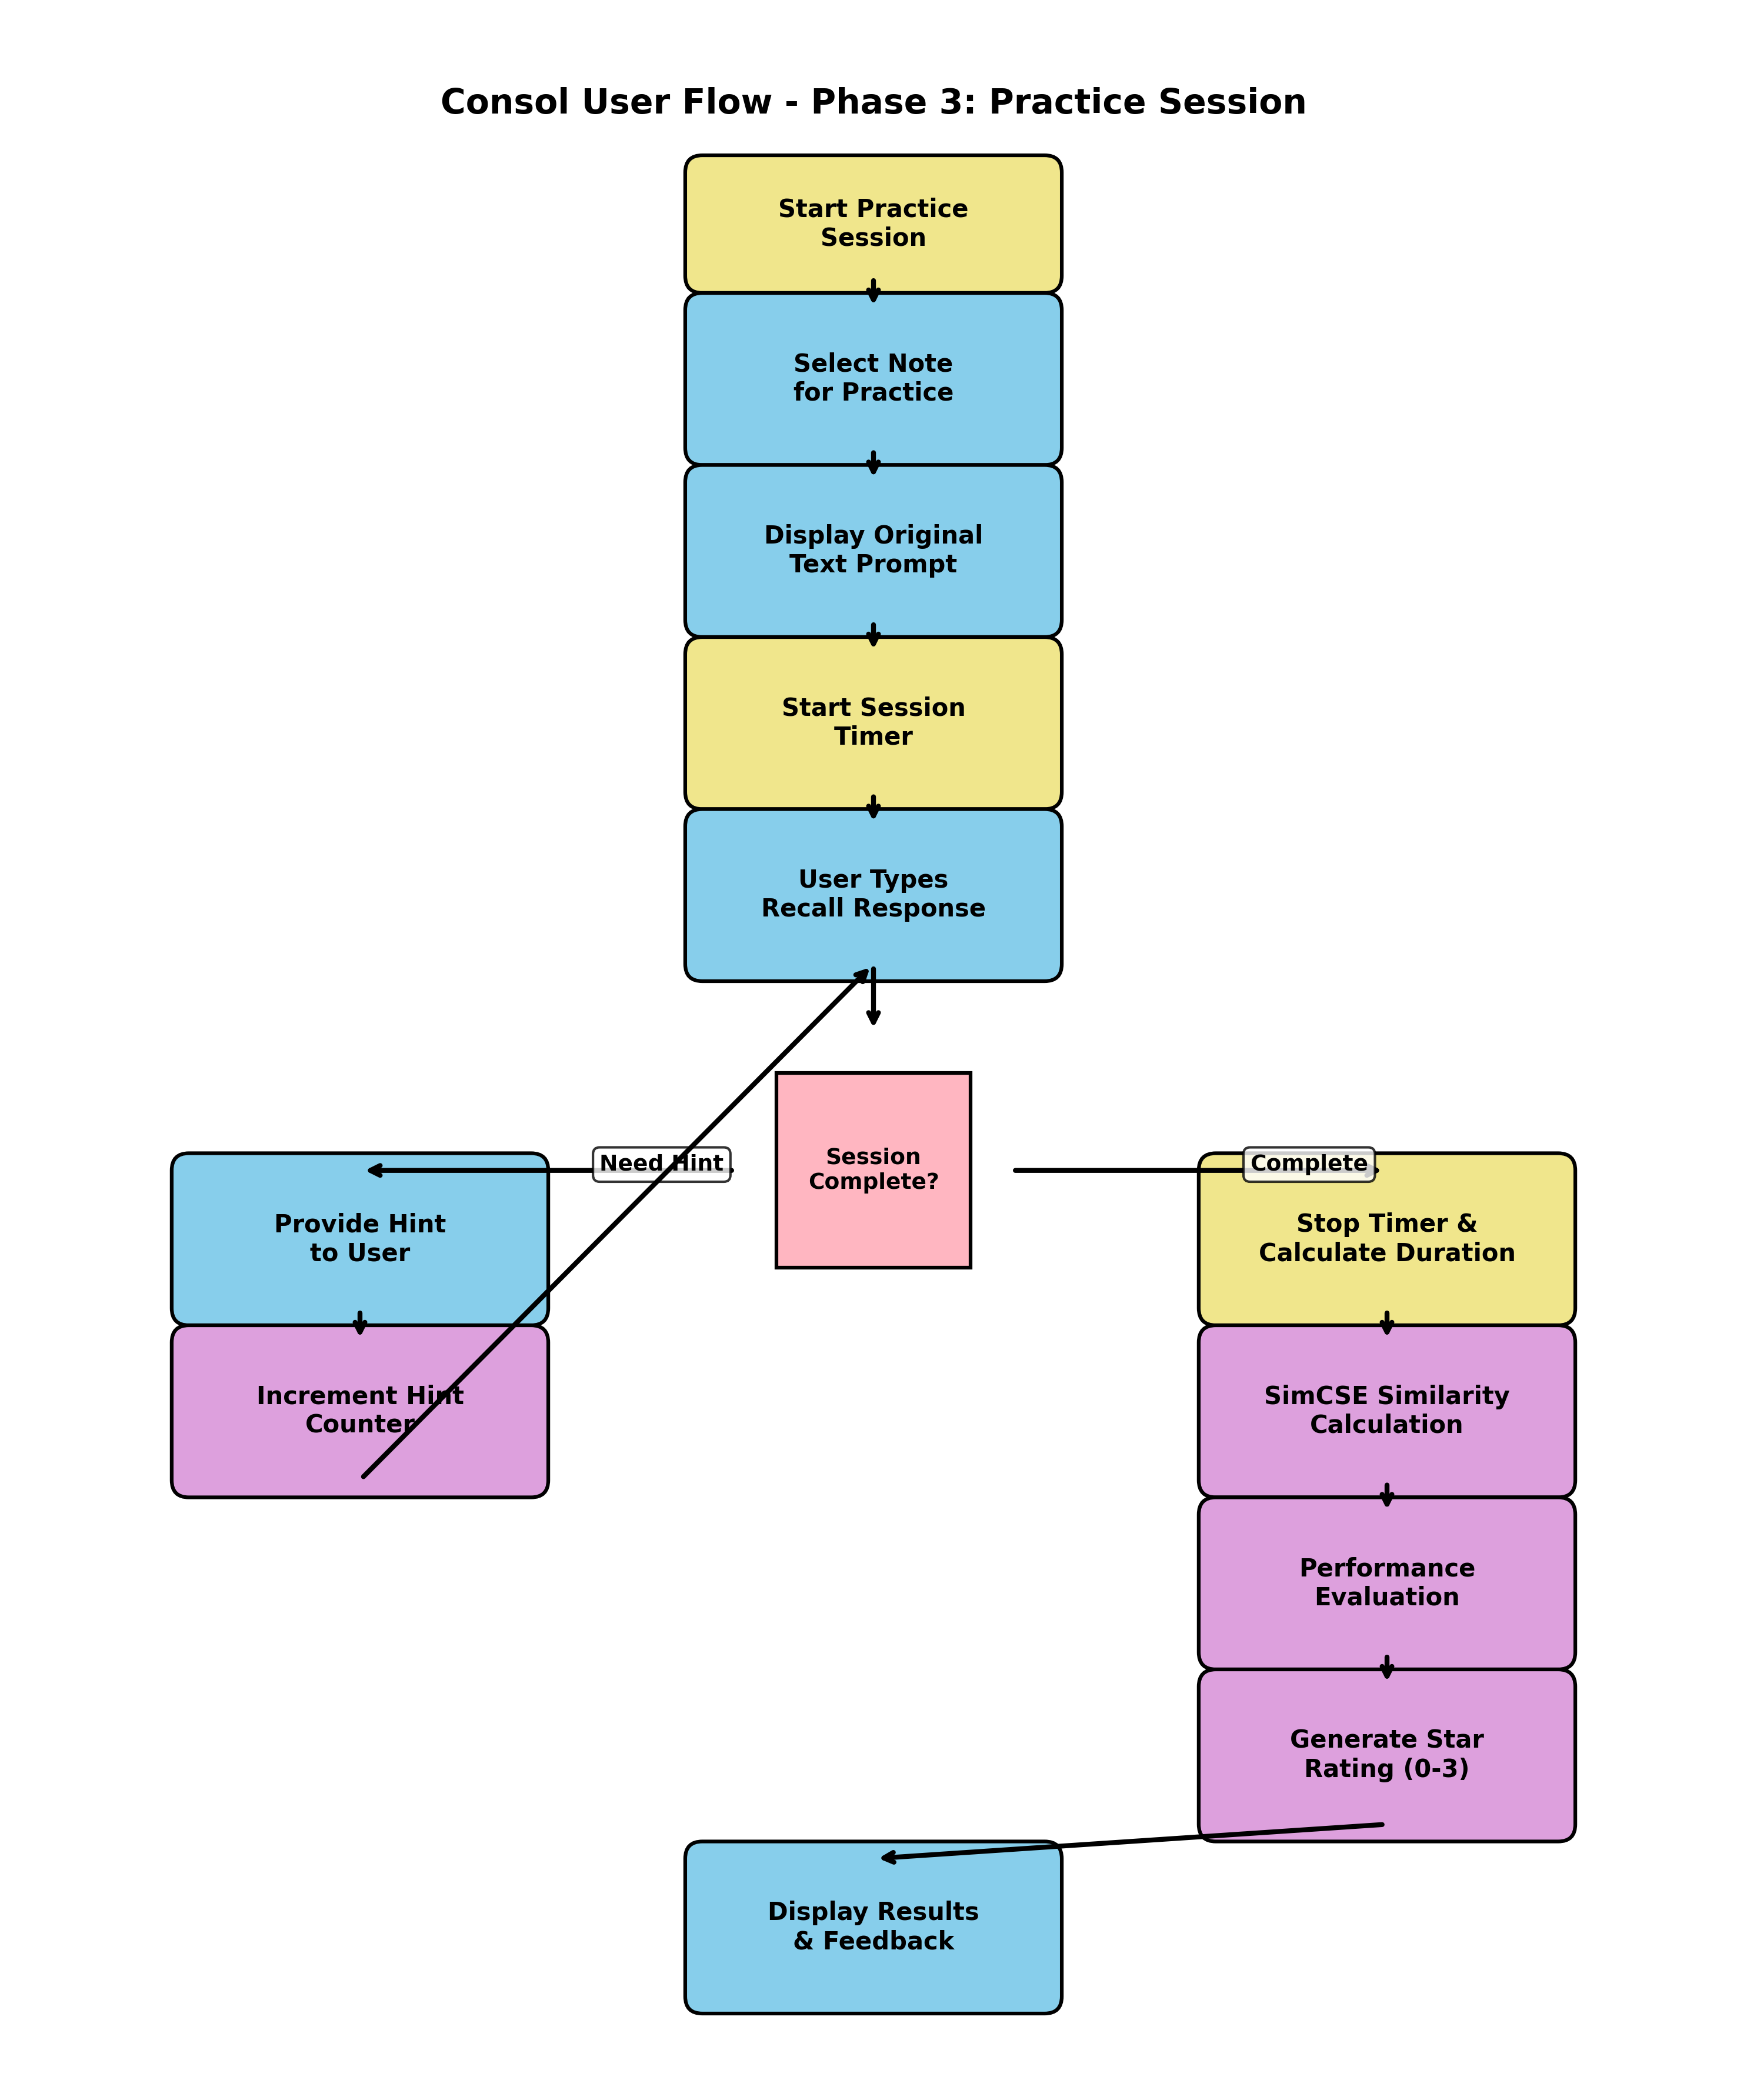
\includegraphics[width=\textwidth]{images/userflow_page3.png}
\caption{User Flow Phase 3: Practice Session Execution}
\label{fig:userflow-phase3}
\end{figure}

\begin{figure}[H]
\centering
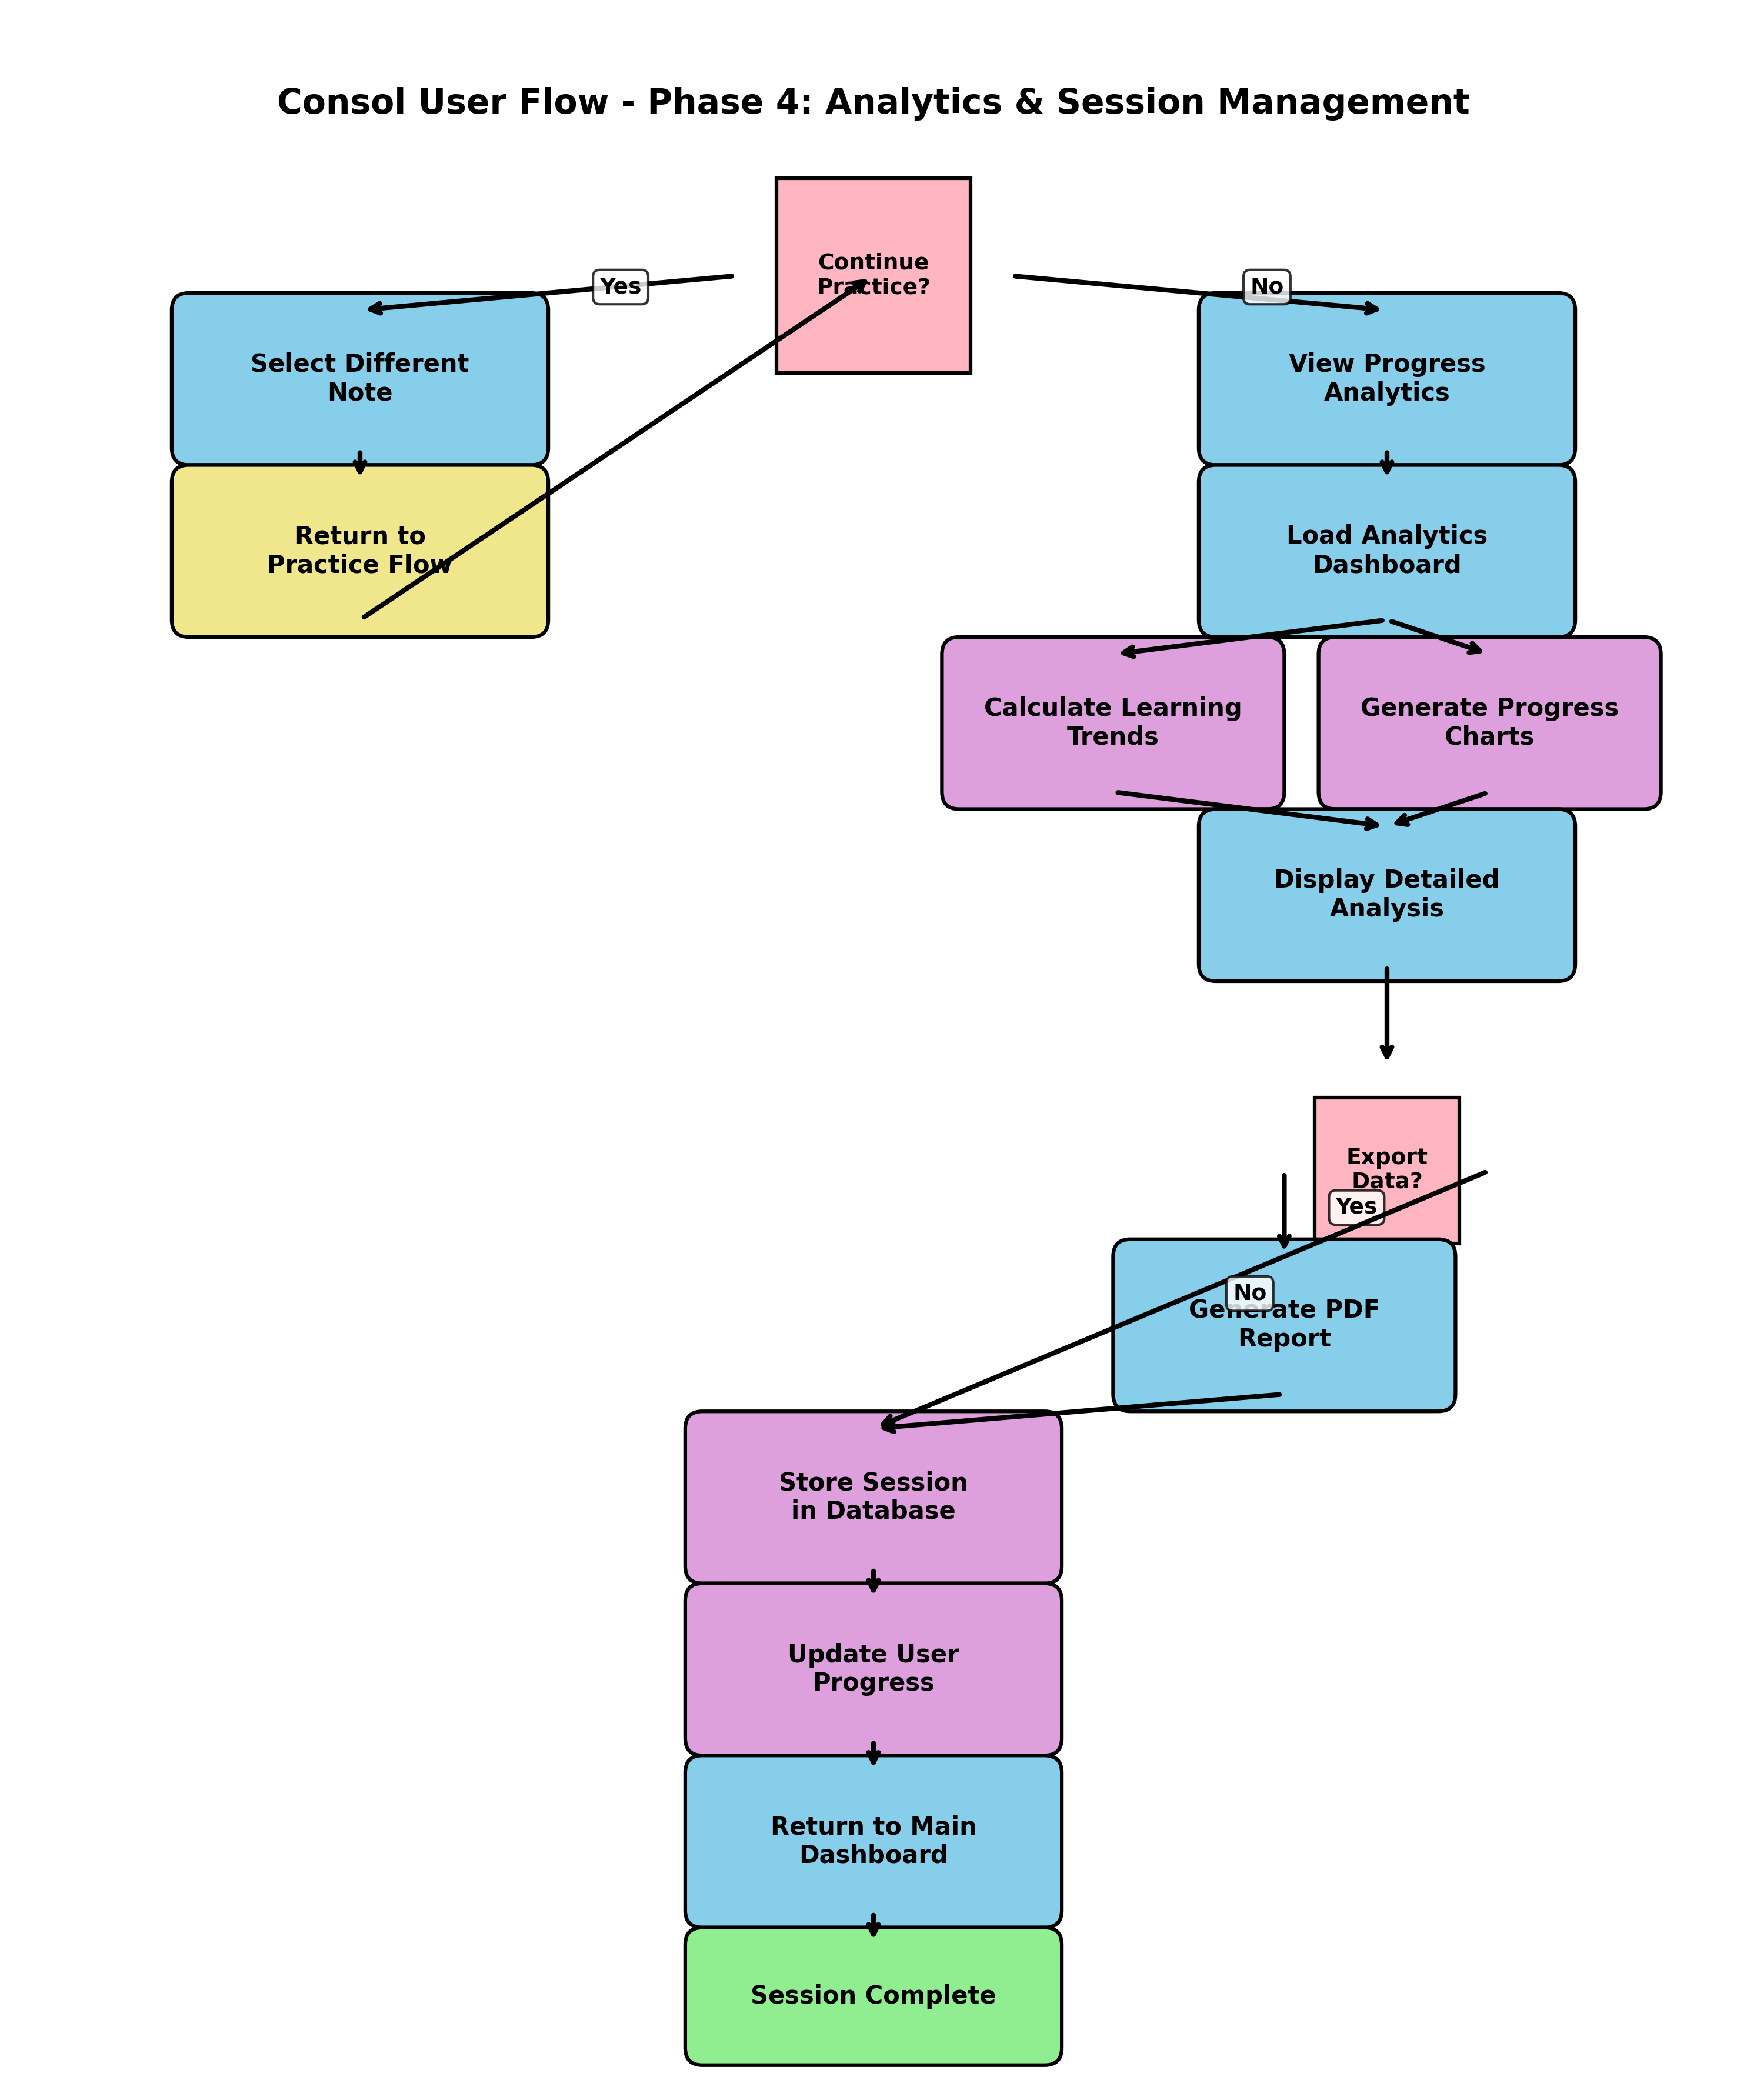
\includegraphics[width=\textwidth]{images/userflow_page4.png}
\caption{User Flow Phase 4: Analytics and Session Management}
\label{fig:userflow-phase4}
\end{figure}

% ==================================================================
% METHOD 3: Single Large TikZ with Landscape Orientation
% ==================================================================

\begin{landscape}
\begin{figure}[H]
\centering
\begin{tikzpicture}[
    node distance=1cm,
    every node/.style={align=center, font=\tiny},
    % ... your TikZ code here for a large horizontal diagram
]
% Large diagram that uses landscape orientation
\end{tikzpicture}
\caption{Complete User Flow - Landscape View}
\label{fig:userflow-landscape}
\end{figure}
\end{landscape}

% ==================================================================
% METHOD 4: Continued Figures Across Pages
% ==================================================================

\begin{figure}[H]
\centering
% First part of the diagram
\begin{tikzpicture}
% ... first section
\end{tikzpicture}
\caption{User Flow - Part 1}
\label{fig:userflow-part1}
\end{figure}

% Text describing the connection

\begin{figure}[H]
\centering
% Second part of the diagram
\begin{tikzpicture}
% ... continuing section
\end{tikzpicture}
\caption{User Flow - Part 2 (continued from Figure \ref{fig:userflow-part1})}
\label{fig:userflow-part2}
\end{figure}

% ==================================================================
% METHOD 5: Using afterpage Package for Complex Layouts
% ==================================================================

% In preamble: \usepackage{afterpage}

\afterpage{
\clearpage
\begin{figure}[p]
\centering
% Large diagram that takes full page
\caption{Full-Page User Flow Diagram}
\end{figure}
\clearpage
}